\chapter{Requisiti}



\section{Utenti del sistema software}
Il software pu\`o rientrare in due categorie:
\begin{itemize}
  \item
    La prima categoria si chiama \emph{auscultazione assistita dal calcolatore}, alla quale afferiscono sistemi di supporto alle decisioni cliniche, progettati per aiutare il medico nella diagnosi attraverso i suoni del corpo. 
    In questo caso gli utenti del sistema fanno parte del personale medico-sanitario di una struttura clinica.
  \item
    La seconda categoria \`e il monitoraggio mobile di segnali biomedici. 
    In questo caso gli utenti del sistema possono essere soggetti privi di conoscenze mediche o infermieristiche.
\end{itemize}

% AGGIUNGERE EVENTUALI:
% who is affected either directly or indirectly? 
% who operates the system (normal and maintenance operators)?
% who benefits from the system (functional, political, financial and social beneficiaries)?
% anyone involved in purchasing or procuring the system
% organizations which regulate aspects of the system (financial, safety, and other regulators)
% people or organizations opposed to the system (negative stakeholders; see also Misuse case)
% organizations responsible for systems which interface with the system under design
% those organizations who integrate horizontally with the organization for whom the analyst is designing the system

\begin{center}
  \begin{figure}
  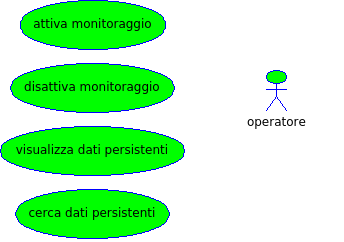
\includegraphics[width=0.5\textwidth,height=0.2\textheight]{./casiDUso.png}
  % casiDUso.png: 339x315 pixel, 96dpi, 8.97x8.33 cm, bb=0 0 254 236
  \caption{Diagramma dei casi d'uso}
  \label{casiDUso}
  \end{figure}
\end{center}



\section{Requisiti funzionali}

% Il software riceve in input il suono registrato sul petto o sulla trachea di soggetti sani o malati e decide la presenza o l'assenza di apnee troppo lunghe in tempo utile. 
% In questo caso il sistema si trova in stato di monitoraggio. 
Il diagramma dei casi d'uso \`e illustrato in figura \ref{casiDUso}:
% Nel seguito ci potremmo riferire alla persona della quale viene monitorato il respiro con il termine \textbf{cliente}. 
I casi d'uso: attiva monitoraggio, visualizza dati persistenti e cerca dati persistenti sono descritti nelle tabelle \ref{casoDUsoMonitoraggio}, \ref{casoDUsoVisualizzaDatiPersistenti} e \ref{casoDUsoCercaDatiPersistenti}. 
% \ref{casoDUsoMonitoraggio}.

   \begin{table}
  \centering
  \begin{tabular}{p{0.17\textwidth} p{0.77\textwidth}}
  \\
  \hline
      Caso d'uso 
    & 
      Attiva monitoraggio
  \\\hline\\
      Attori
    &
      C'\`e un solo attore attivo: un soggetto che intende monitorare il proprio respiro oppure un membro del personale medico sanitario che intende monitorare il respiro di un paziente. Il soggetto del quale si misura il respiro \`e un attore passivo in questo caso d'uso perch\'e in generale esso pu\`o evitare di interagire in modo attivo col sistema stesso. 
  \\
      Precondizioni
    &
      \begin{itemize}
	\item 
	  Lo stetoscopio elettronico \`e stato installato correttamente sul torace del soggetto o sulla trachea del soggetto.
	\item
	  I dispositivi di interfaccia tra lo stetoscopio e il sistema sono configurate correttamente.
      \end{itemize}
  \\
      Sequenza principale degli eventi
    &
      \begin{enumerate}
	\item 
	  L'attore attiva il sistema di monitoraggio attraverso l'interfaccia utente. 
	  In questo passo l'attore specifica se intende memorizzare o meno i dati e in che forma.
	  L'attore pu\`o specificare la soglia di allarme per l'apnea.
	\item
	  Il sistema stabilisce una connessione con lo stetoscopio elettronico. 
	  Se questo passo fallisce allora comincia la sequenza alternativa degli eventi.
	\item	
	  Il sistema passa in fase di monitoraggio.
	\item
	  Se la frequenza di respirazione scende al disotto di una certa soglia critica, il sistema lo segnala attraverso una parte dedicata dell'interfaccia utente, ad esempio un segnale acustico.
      \end{enumerate}      
  \\
      Sequenza alternativa degli eventi
    &
      \begin{enumerate}
	\item 
	  Il sistema segnala un errore appropriato attraverso l'interfaccia utente.
      \end{enumerate}      
  \\
      Postcondizioni
    &
      Il sistema di monitoraggio \`e attivo. 
  \\\\
  \hline
  \end{tabular}
   \caption{Caso d'uso: attiva monitoraggio}
   \label{casoDUsoMonitoraggio}
   \end{table}




   \begin{table}
\centering
  \begin{tabular}{p{0.17\textwidth} p{0.77\textwidth}}
  \\
  \hline
      Caso d'uso 
    & 
      Visualizza dati persistenti
  \\
  \hline\\
      Attori
    &
      C'\`e un solo attore ed \`e l'operatore del sistema. In questo caso d'uso un utente pu\`o consultare i dati relativi ai monitoraggio passati. 
  \\
      Precondizioni
    &
      L'utente conosce le chiavi di accesso ai dati: nome del soggetto e data.
%       \begin{itemize}
% 	\item 
%       \end{itemize}
  \\
      Sequenza principale degli eventi
    &
      \begin{enumerate}
	\item 
	  L'attore inserisce nome del soggetto e/o data nella parte dell'interfaccia utente dedicata alla visualizzazione dei dati persistenti.
	\item
	  Il sistema visualizza i dati relativi alle chiavi inserite, se queste sono corrette. Altrimenti visualizza un messaggio di errore.
% 	\item	
% 	  Se ci sono risultati e l'attore ne seleziona uno, il sistema lo visualizza nella forma specificata dall'interfaccia utente. Un modo per visualizzare i dati potrebbe essere un grafico che ha il tempo sulle ordinate e la frequenza respiratoria sulle ascisse.
      \end{enumerate}      
  \\
      Postcondizioni
    &
      -
  \\\\
  \hline
  \end{tabular}
   \caption{Caso d'uso: visualizza dati persistenti}
   \label{casoDUsoVisualizzaDatiPersistenti}
   \end{table}



   \begin{table}
  \centering
  \begin{tabular}{p{0.17\textwidth} p{0.77\textwidth}}
  \\
  \hline
      Caso d'uso 
    & 
      Cerca dati persistenti
  \\
  \hline\\
      Attori
    &
      Utente del sistema. In questo caso d'uso un utente pu\`o cercare i dati relativi ai monitoraggio passati. Le chiavi di ricerca sono il nome del soggetto e la data.
  \\
      Precondizioni
    &
      -
%       \begin{itemize}
% 	\item 
%       \end{itemize}
  \\
      Sequenza principale degli eventi
    &
      \begin{enumerate}
	\item 
	  L'attore inserisce nome del soggetto e/o data nella parte dell'interfaccia utente dedicata alla ricerca dei dati persistenti.
	\item
	  Il sistema visualizza i risultati della ricerca.
% 	\item	
% 	  Se ci sono risultati e l'attore ne seleziona uno, il sistema lo visualizza nella forma specificata dall'interfaccia utente. Un modo per visualizzare i dati potrebbe essere un grafico che ha il tempo sulle ordinate e la frequenza respiratoria sulle ascisse.
      \end{enumerate}      
  \\
      Postcondizioni
    &
      -
  \\\\
  \hline
  \end{tabular}
   \caption{Caso d'uso: cerca dati persistenti}
   \label{casoDUsoCercaDatiPersistenti}
   \end{table}





\section{Requisiti funzionali opzionali}

Il sistema pu\`o essere arricchito con i requisiti illustrati in figura \ref{opt}. I casi d'uso: visualizza flusso e invia dati sono descritti nella tabelle \ref{visualizzaFlusso} e \ref{inviaDati}.


\begin{figure}
 \centering
 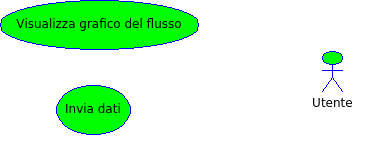
\includegraphics[width=0.4\textwidth]{./opt.png}
 % opt.png: 382x147 pixel, 96dpi, 10.11x3.89 cm, bb=0 0 286 110
  \caption{Diagramma dei casi d'uso opzionali}
\label{opt}
\end{figure}



  \begin{table}
  \centering
  \begin{tabular}{p{0.17\textwidth} p{0.77\textwidth}}
  \\
  \hline
      Caso d'uso 
    & 
      Visualizza flusso
  \\
  \hline\\
      Attori
    &
      Utente del sistema. 
  \\
      Precondizioni
    &
      -
%       \begin{itemize}
% 	\item 
%       \end{itemize}
  \\
      Sequenza principale degli eventi
    &
      In questo caso d'uso il sistema riconosce la localizzazione nel tempo degli eventi inspiratori ed espiratori e visualizza un grafico che ha il tempo sulle ascisse e il valore stimato del flusso sulle ordinate. Nello standard SI un flusso d'aria si misura in litri al secondo. Non \`e necessario stimare il valore oggettivo del flusso ma basta usare valori significativi in modo relativo al flusso massimo e al flusso nullo.
  \\
      Postcondizioni
    &
      -
  \\\\
  \hline
  \end{tabular}
   \caption{Caso d'uso: visualizza flusso}
   \label{visualizzaFlusso}
   \end{table}





   \begin{table}
  \centering
  \begin{tabular}{p{0.17\textwidth} p{0.77\textwidth}}
  \\
  \hline
      Caso d'uso 
    & 
      Invia dati.
  \\
  \hline\\
      Attori
    &
      Utente del sistema. 
  \\
      Precondizioni
    &
      L'utente conosce le chiavi di accesso ai dati e l'URL del personale medico sanitario.
%       \begin{itemize}
% 	\item 
%       \end{itemize}
  \\
      Sequenza principale degli eventi
    &
      \begin{enumerate}
	\item
	  L'utente inserisce le chiavi di accesso ai dati e l'URL del personale medico sanitario nella parte dell'interfaccia utente dedicata a questo caso d'uso.
	\item
	  Il sistema invia i dati e mostra il risultato dell'operazione (successo o fallimento con messaggio d'errore significativo).
      \end{enumerate}
  \\
      Postcondizioni
    &
      -
  \\\\
  \hline
  \end{tabular}
   \caption{Caso d'uso: invia dati}
   \label{inviaDati}
   \end{table}




% \begin{itemize}
%   \item 
%     Distinguere l'inspirazione dall'espirazione e stimare il flusso d'aria.
%   \item	
%     Classificare la respirazione in alcune categorie. Ad esempio distinguere una respirazione normale da una respirazione in presenza di patologie dell'apparato respiratorio e in alcuni casi capire di che malattia si tratta.
% %   \item
% %     Usare un segnale acustico per segnalare condizioni patologiche di emergenza: ad esempio apnea troppo lunga o respirazione di Cheyne-Stokes.
% %   \item
% %     Avere un meccanismo di persistenza dei dati ad esempio un insieme di file in un memoria fissa, un server dedicato o un database remoto o locale.
%   \item
%     Nel caso di home monitoring, offrire la possibilit\`a di inviare i dati ad una struttura sanitaria.
% \end{itemize}

\section{Requisiti non funzionali}

\subsubsection{Sistemi real time}
\cite{RealTime} e \cite{WikiRealTime} danno le seguenti definizioni. Diciamo che un sistema \`e in \emph{tempo reale} o \emph{real time} se la correttezza dell'output dipende anche dal tempo impiegato per calcolarlo. I sistemi real time hanno delle scadenze entro le quali devono dare una risposta. Possiamo classificare i sistemi real time in base alle conseguenze subite dalla mancanza di una risposta entro la scadenza prevista:
\begin{description}
  \item[$hard$]
    Non rispettare una scadenza \`e un errore fatale. 
% Quindi il compito di un sistema real time hard \`e quello di assicurarsi che tutte le scadenza siano rispettate. Nei sistemi real time hard le scadenze devono essere rispettate altrimenti le conseguenze potrebbero essere gravi per le persone o cose di valore. 
  \item[$firm$]
    In questo caso si possono tollerare frequenti mancanze nel rispetto delle scadenze, ma queste mancanze possono degradare la qualit\`a del servizio.
  \item[$soft$]
    Per i sistemi real time soft, l'obiettivo diventa quello di rispettare un certo sottoinsieme di scadenze con lo scopo di ottimizzare alcuni criteri che dipendono dall'applicazione. 
% Il criterio di ottimizzazione particolare dipende dall'applicazione, ad esempio: massimizzare il numero di scadenze soddisfatte o minimizzare il ritardo. 
\end{description}

% In the context of multitasking systems the scheduling policy is normally priority driven (pre-emptive schedulers). Other scheduling algorithms include Earliest Deadline First, which, ignoring the overhead of context switching, is sufficient for system loads of less than 100\%.[2] New overlay scheduling systems, such as an Adaptive Partition Scheduler assist in managing large systems with a mixture of hard real-time and non real-time applications.


% Consider an audio DSP example: if a process requires 2.01 seconds to analyze, synthesize, or process 2.00 seconds of sound, it is not real-time. If it takes 1.99 seconds, it is or can be made into, a real-time DSP process.

\subsubsection{Caratteristiche real time del sistema}

In un sistema real time di elaborazione di segnali digitali, il segnale in input pu\`o essere virtualmente illimitato nel tempo. In realt\`a dei valori che massimizzano la durata del segnale si potrebbero trovare ma sono abbastanza grandi da costringerci ad usare una particolare definizione di scadenze temporali. 
Il ritardo nell'elaborazione deve essere limitato anche se il processo continua per un tempo illimitato. Quindi consideriamo la media del tempo di elaborazione del segnale per campione di segnale in un intervallo di tempo abbastanza piccolo rispetto ai vincoli real time, ad esempio un secondo. Questa media non deve essere maggiore del periodo di campionamento. Questo criterio vale sia che il segnale venga esaminato in blocchi sia che il segnale venga esaminato campione per campione\cite{RTDSPIA}.
In altre parole un sistema real time di elaborazione di un segnale virtualmente illimitato deve avere un tempo di esecuzione per secondo di segnale, minore di un secondo.


La velocit\`a di esecuzione un algoritmo \`e una grandezza data dal rapporto tra la dimensione dell'input e il tempo di esecuzione su di esso.
In questo caso la dimensione dell'input \`e la durata del segnale e non ci interessa la velocit\`a calcolata su tutto il segnale di input ma quella calcolata ad intervalli regolari di dimensione piccola rispetto ai vincoli real time.
Quindi si pu\`o definire la velocit\`a $v$ del processo come la quantit\`a di campioni che ci sono in un secondo di segnale, fratto il tempo impiegato per l'elaborazione di un secondo di segnale. 
In un secondo di segnale ci sono un numero di campioni pari alla frequenza di campionamento del segnale $f_{c} Hz$.
% Siamo abituati a pensare alla velocit\`a come ad una misura di spazio fratto una misura di tempo e quindi pu\`o sembrare controintuitivo misurare la velocit\`a in secondi al secondo ma in questo caso la dimensione dell'input \`e calcolabile in secondi.
Il sistema pu\`o calcolare tale velocit\`a ogni secondo e quindi produrre una sequenza di velocit\`a $v_{1}, v_{2}, \cdots $. 
Una condizione necessaria affinch\'e il sistema si trovi sempre (ogni secondo) in uno stato valido \`e la seguente:
\[
  \forall n.\; v_{n} \geq f_{c}
\]

% Si definisce il ritardo globale relativo al tempo $n$ (calcolato in secondi) come 
% \[
%   r_{g}(n)=f_{c} \cdot n  - 1s \cdot \displaystyle\sum_{i=1}^{n} v_{i} 
% \]
% ed \`e significativo solo se \`e positivo, altrimenti significa che il sistema non ha accumulato ritardo al tempo $n$. Il ritardo globale ha come unit\`a di misura il numero di campioni. Il ritardo $r_{g}$ si traduce in un tempo di ritardo in secondi pari a 
% \[
%   \displaystyle \frac{r_{g}}{f_{c}}
% \]
% nell'ipotesi che il sistema processi il segnale in blocchi di un secondo.

Il sistema in fase di monitoraggio deve segnalare la presenza di apnee troppo lunghe. In particolare consideriamo troppo lunga una apnea di $30$ secondi. Partiamo dall'assunto che le sole scadenze siano quelle relative all'evento apnea troppo lunga e che non rispettare una scadenza significa non dare l'allarme in tempo prima che il soggetto rischi gravi problemi cardiorespiratori. Allora ci troviamo in presenza di un sistema real time hard. Tuttavia i vincoli di tempo per le scadenze sono blandi relativamente ai tempi di esecuzione che si possono prevedere su un calcolatore moderno.

% Una condizione sufficiente affinch\'e il sistema si trovi in uno stato di errore \`e che il ritardo globale superi i $30s \cdot f_{c} Hz$ campioni. 

























\section{Requisiti non funzionali opzionali}
Il software deve funzionare bene anche in presenza di rumore. 



\section{Scelta della soglia di allarme}

La soglia oltre la quale una apnea \`e considerata pericolosa deve essere configurabile.
Il valore soglia deve essere stabilito da personale medico qualificato.
Si pu\`o intuire che una soglia troppo bassa potrebbe degradare la qualit\`a del sonno del soggetto in un modo patogenico o quantomeno in un modo tale da rendere inutile il monitoraggio.
Al contrario una soglia troppo alta espone il soggetto ad un rischio troppo elevato.
Ci si pu\`o aspettare che la soglia di allarme non sia oggettiva ma debba essere personalizzata e che vari con l'et\`a e alcuni parametri fisiologici del soggetto.




